% proposal.tex
\documentclass[main.tex]{subfiles}
\begin{document}
\chapter{Prediction of Mechanical Properties through Machine Learning} \label{ch:ml}

\section{Foreword} \label{sec:fw_ml}

The use of AM technologies to produce small batches of highly customized, complex parts in a reduced development cycle results extremely attractive to all industries. However, for AM parts to be fully adopted in industrial scenarios, engineers have to be able to confidently assess the structural integrity of the finished part under its intended loading conditions. This requirement is unfortunately not fully possible at the time this work was produced, partly because the mechanical properties of AM tend to be anisotropic, and partly because the relationships that exist between processing parameters, underlying physics of the process, and final mechanical part properties aren't fully comprehended. However, these obstacles present an interesting case for the application of Machine Learning (ML) techniques, where the inputs and outputs of a particular phenomenon are known, but there's a lack of explicit rules that indicate a relationship between the two. 

This work uses the Fused Filament Fabrication (FFF) process as a case study for the application of ML techniques to predict the final mechanical properties of a printed part. Experimental work involved producing a variety of tensile coupons, developed under various printing conditions, and where the filament extrusion speed, filament extrusion force, and printing temperature were measured in real time using machines fitted with in-line sensors. These specimens were then tested up to tensile failure, and the collective data of printing parameters, measured process indicators, and mechanical tests results were used to train a Neural Network capable of predicting the tensile failure stress.

In the context of this dissertation, this represents an alternative method for part failure prediction to construction and evaluation of a failure envelope. However, it should be noted that both methods are not mutually exclusive, and as will be discussed under future work, the author believes they can be combined quite well. 

\section{Introduction} \label{sec:ml_intr}

The set of printing conditions that lead to an optimal part in terms of mechanical properties aren't still fully comprehended. However, if there existed an FFF machine with in-line sensors that allowed monitoring a variety of process-variables, as well as data generated from mechanical tests and ancillary experiments, this would constitute an interesting case for development of a Machine Learning (ML) system. These excel in cases where the inputs and outcomes of a particular phenomena or task are known, but connecting the two through an explicit set of rules or relationships can result extremely complex and time consuming \cite{Chollet2018}. In this manner, ML models are \emph{trained}, as opposed to explicitly programmed, as illustrated in Figure \ref{fig:MLvsP}, where the differences between ML and traditional programming philosophies are compared. 

\begin{figure}[!htbp]
	\center
	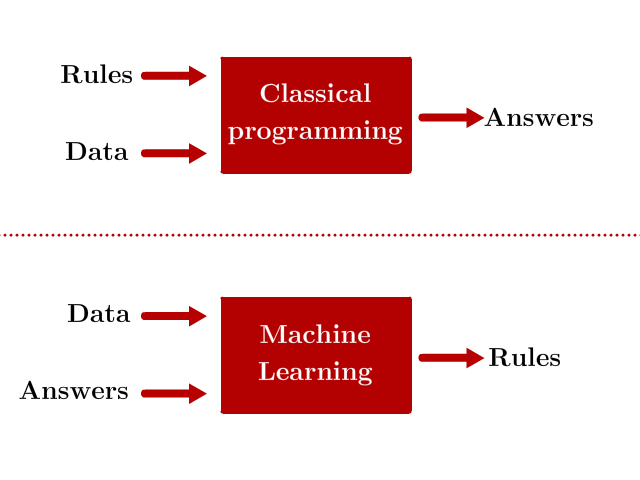
\includegraphics[height=6cm]{ML}
	\caption{Differences between traditional programming and machine learning. \cite{Chollet2018}} \label{fig:MLvsP_2}
\end{figure}

The potential to apply ML solutions in the field of AM has been noted by several authors \cite{Razvi2019,Meng2020}. Example cases include design-recommendation systems, topology optimization solutions, tolerancing and manufacturability assessment, and material classification and selection \cite{Razvi2019}. The specific algorithm applied for each case varied wildly depending on the nature of the task, but in general, Support Vector Machines (SVM) and Neural Networks (NN) appear to be the most prevalent solutions.

A Neural Network (NN) algorithm is effectively a facsimile of how biological neurons establish connections and communications with each other. In summary, the inputs of the problem are fed to a layer of nodes, or "neurons". Each node has itself a variety of connections to other neurons, and an associated weight and activation threshold, which if surpassed, triggers information transfer to its connections in nodes waiting in subsequent layers. Finally, the information reaches the network stratus that estimates the outcome of whatever phenomena the model is trying to characterize, traditionally named the output layer \cite {Chollet2018, IBMCloudEducation2020, Geron2019}. The weights and activation thresholds of each node are iteratively tuned as the NN architecture is exposed to a training data set, while being compared to a separate set of data points used for validation. Once the accuracy of the model reaches its desired value, the underlying communication between the neurons is capable of making predictions based on what the input layer is perceiving. A schematic of a NN can be seen in Figure \ref{fig:NN}. This particular NN is called a Deep Neural Network, as the number of layers of nodes surpasses three \cite{IBMCloudEducation2020}. This type of architecture tends to be reserved for computationally complex tasks, such as text recognition or image processing.  

\begin{figure}[!htbp]
	\center
	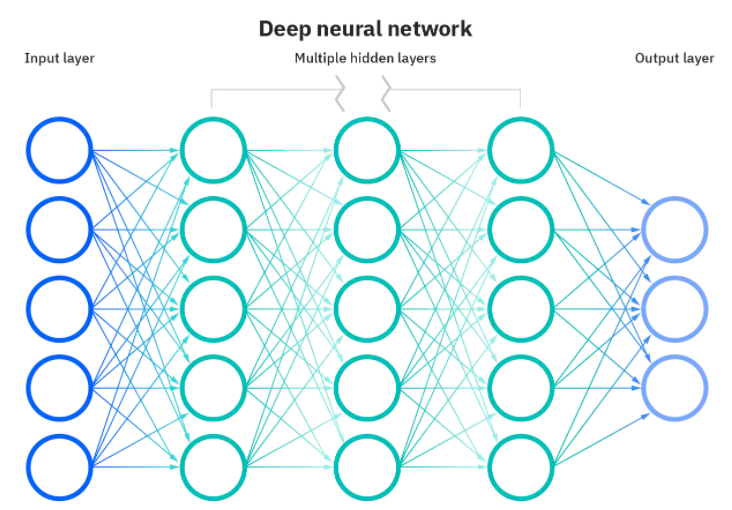
\includegraphics[width=0.9\linewidth, keepaspectratio]{NN_scheme}
	\caption{Schematic of a NN \cite{IBMCloudEducation2020}} \label{fig:NN}
\end{figure}



Given the factors outlined this far, the fundamental goal of this research is to predict FFF part mechanical performance by finding relations between processing conditions and strength through the use of sensors and machine learning. The success of this project would allow design engineers to confidently assess if a part manufactured through FFF will meet the mechanical requirements imposed by its intended application. This work proposes developing and using a modified printer with force and print speed sensors, as well as mechanical testing and $\mu$CT scans to generate data that can be used to train a predictive tool based on ML. This tool can then be used to predict final mechanical properties of the part based on the data generated during the print. This ML system would accept filament dimensions, printing temperature, filament force, filament velocity, print orientation, layer height, or any subset of these items as inputs, and produce final part porosity and/or mechanical strength in a particular load direction as outputs. These parameters were chosen based on previous work performed by Koch, Van Hulle and Rudolph \cite{Koch2017}, where the final tensile strength of FFF coupons was shown to be related to the morphology of the printed bead, which is significantly affected by processing parameters and variations in the volumetric output of the nozzle; research published by Sood \emph{et al.} \cite{Sood2012} where a NN was able to predict the compressive strength of FDM parts with an $R^2= 0.9977$ using layer thickness, raster angle, orientation, raster width, and air gap as inputs; as well as the proposed FFF melting models established by Bellini \emph{et al.} \cite{Bellini2004} and Osswald \emph{et al.} \cite{OsswaldMelting18}. The specifics of the architecture of the ML system are still under development, as it may prove useful to segment the problem into several sub-systems connected in series, in what is called a machine learning \emph{pipeline} \cite{Geron2019}. However, given the specifics of the task, one can conclude that the system will involve supervised learning applied to a regression problem, given that all the inputs to the system will consist of pre-selected attributes, and the mechanical response and/or porosity of a printed part can be treated as a target value the ML system has to be able to predict \cite{Mohammed2017, Meng2020}.


\section{Experimental Methods} \label{sec:ml_meth}

\subsection{Feature Selection and Engineering} \label{ssec:ml_fs}
\begin{figure}[!htbp]
	\center
	\includegraphics[height=7cm]{forcesetup}
	\caption{Schematic of modified FFF printer with sensors} \label{fig:shakira}
\end{figure}

\begin{figure}[!htbp]
	\center
	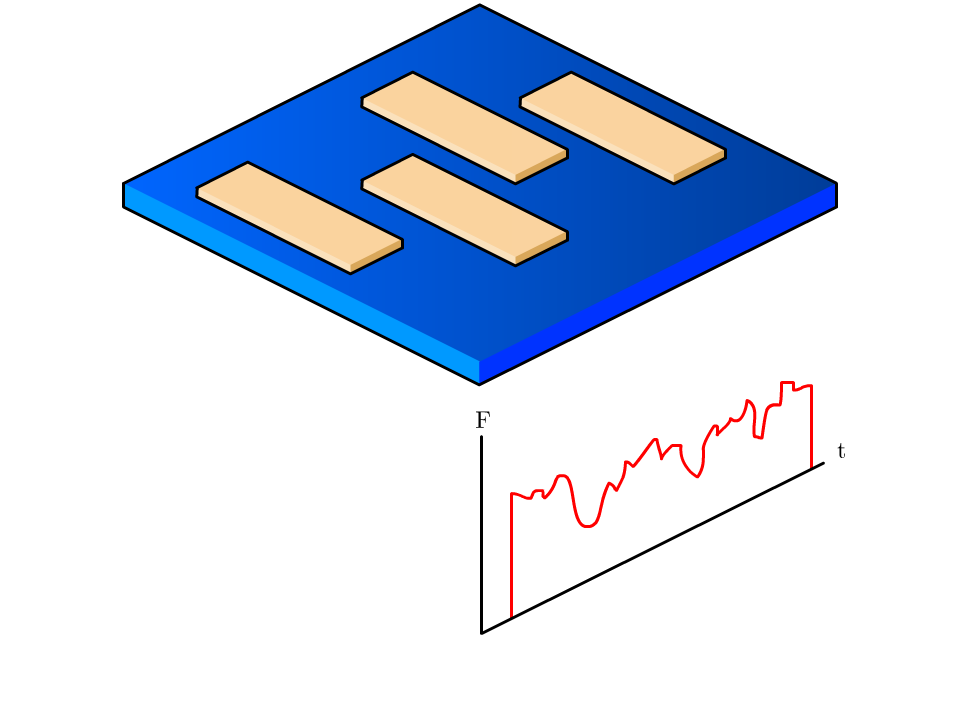
\includegraphics[height=8cm]{coupon_print_diagram}
	\caption{Schematic of print experiment} \label{fig:print_dia}
\end{figure}

\begin{figure}[!htbp]
	\center
	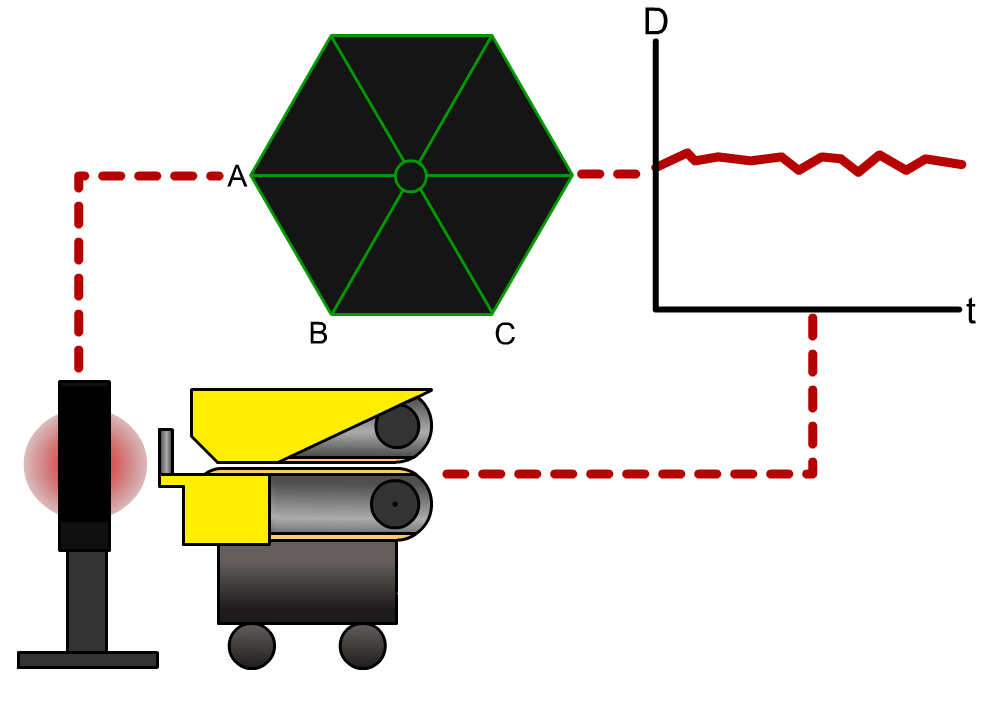
\includegraphics[width=0.6\linewidth]{filament_measurement}
	\caption{Filament geometry information, acquired through a laser micrometer } \label{fig:FD}
\end{figure}

\begin{figure}[h]
	\center
	\subfloat[Effect of diameter on measured filament speed \label{fig:D_sp}]{%
		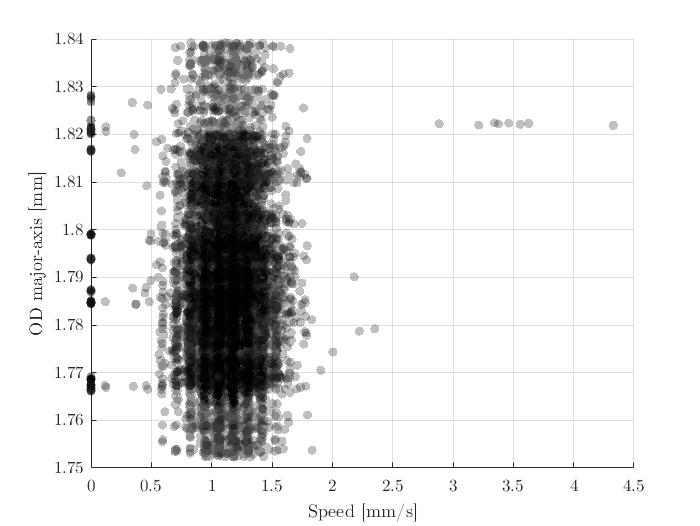
\includegraphics[width=0.8\linewidth, keepaspectratio]{speed-OD}
	}
	\linebreak
	\subfloat[Effect of diameter on measured filament force \label{fig:D_f}]{%
		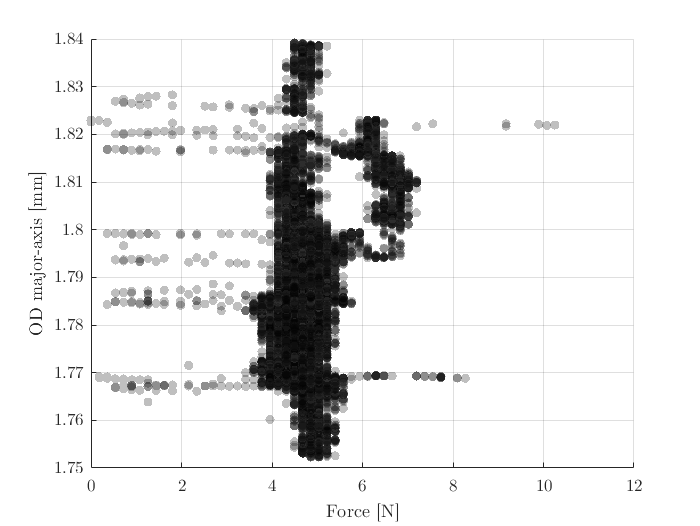
\includegraphics[width=0.8\linewidth, keepaspectratio]{force-OD}
	}
	\caption{Effect of diameter on filament force and speed} \label{fig:dia_f_sp}
\end{figure}

\begin{figure}[h]
	\center
	\subfloat[Effect of ovality on measured filament speed \label{fig:O_sp}]{%
		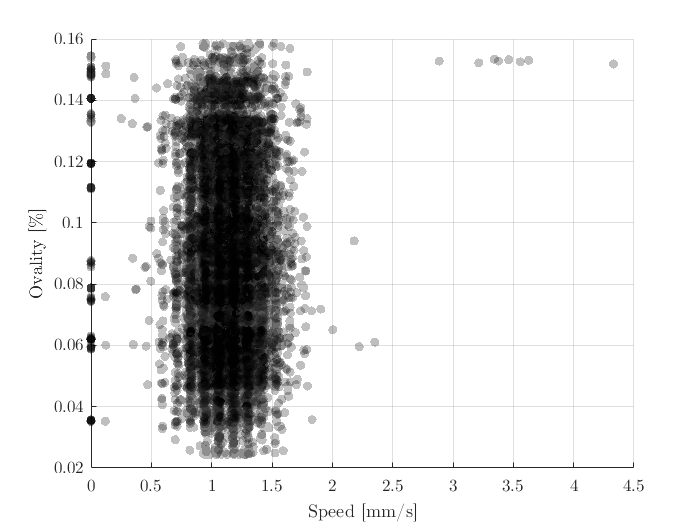
\includegraphics[width=0.8\linewidth, keepaspectratio]{speed-ovality}
	}
	\linebreak
	\subfloat[Effect of ovality on measured filament force \label{fig:O_f}]{%
		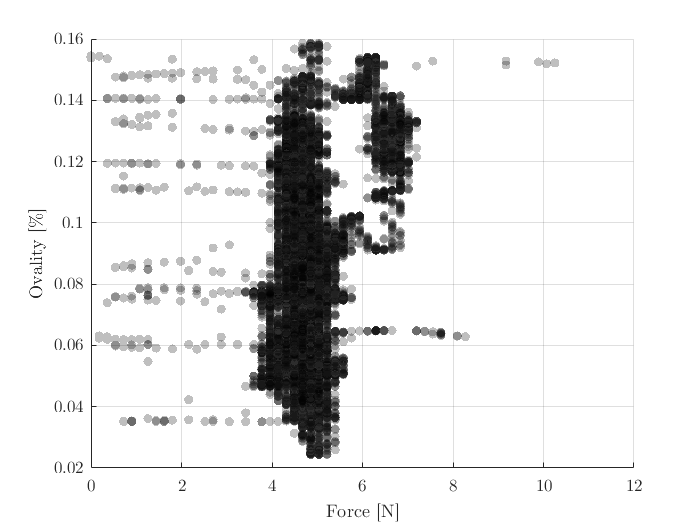
\includegraphics[width=0.8\linewidth, keepaspectratio]{force-ovality}
	}
	\caption{Effect of diameter on filament force and speed} \label{fig:ov_f_sp}
\end{figure}

\subsection{Data generation and preparation}\label{ssec:datag}

\subsection{ML system architecture, training, and validation}\label{ssec:MLA}

The following step of this work would involve using small subsets of the training data to test multiple models and algorithms in a reasonable amount of time. Performance metrics such as the Mean Square Error (MSE) or the Mean Absolute Error (MAE) would help narrow down the optimal candidate for each task \cite{Geron2019}. Depending on the outcome, the final architecture of the predictive system will be decided, including the algorithms for each segment of the machine learning pipeline if applicable. Ultimately, the final architecture of the system will be trained using the training data, and benchmarked against the validation set to check for inherent issues to the ML field, such as overfitting, and to assess the validity of the predicted outcome. The programming language of choice will be \emph{Python 3}, given its relative ease of syntax, open-source nature, as well as the availability of data science and ML libraries and resources such as \emph{NumPy, pandas, and TensorFlow}.


%______________________________________________________________________________________________
% Nomenclature introduced in this chapter:
\nomenclature[A]{ML}{Machine Learning}% 
\nomenclature[A]{SVM}{Support Vector Machines}%
\nomenclature[A]{NN}{Neural Network}%
\nomenclature[A]{MSE}{Mean Square Error}%
\nomenclature[A]{MAE}{Mean Absolute Error}%

% Symbols introduced in this chapter:
%\nomenclature[S]{$X_t$}{Tensile strength in the 1-1 direction \nomunit{$MPa$}}
\end{document}